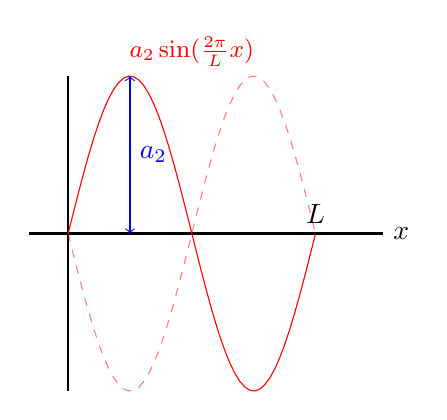
\begin{tikzpicture}
% Axis
\draw[thick] (-.5,0)--(4,0) node[right]{$x$};
\draw[thick] (0,-2)--(0,2) node[above]{ };

\draw[red, samples=50, domain=0:pi] plot ({\x},{2*sin(2* \x r)});
\draw[red, samples=50, domain=0:pi, dashed, opacity=0.5] plot ({\x},{2*-sin(2 * \x r)});

\node[above, red] at (pi/2,2) {\small $a_2 \sin(\frac{2\pi}{L}x)$};

\draw[<->,blue, samples=50] (pi/4,0) -- (pi/4,2) node[right, pos=0.5]{$a_2$};

\node[above] at (pi,0) {$L$};

\end{tikzpicture}
